%
% This is the LaTeX template file for lecture notes for CS3200,
% Computer Netoworks.  When preparing LaTeX notes for this class, please use this template.
%

\documentclass[twoside]{article}

\usepackage{setspace}       % 1.5 spacing
% \usepackage{psfig,epsfig}
\usepackage{multicol}
\usepackage{subfigure}
\usepackage{epsfig,color}
\usepackage{hyperref}
\hypersetup{
    colorlinks=true,
    linkcolor=black,
    % filecolor=magenta,      
    urlcolor=blue,
}
\usepackage{graphics}
\usepackage{hyperref}
\usepackage{multirow}
\usepackage{amsfonts}
\usepackage{amsmath}
\setlength{\oddsidemargin}{0.25 in}
\setlength{\evensidemargin}{0.25 in}
\setlength{\topmargin}{-0.6 in}
\setlength{\textwidth}{6.5 in}
\setlength{\textheight}{8.5 in}
\setlength{\headsep}{0.75 in}
\setlength{\parindent}{0 in}
\setlength{\parskip}{0.1 in}

%
% The following commands set up the lecnum (lecture number)
% counter and make various numbering schemes work relative
% to the lecture number.
%
\newcounter{lecnum}
\renewcommand{\thepage}{\thelecnum-\arabic{page}}
\renewcommand{\thesection}{\thelecnum.\arabic{section}}
\renewcommand{\theequation}{\thelecnum.\arabic{equation}}
\renewcommand{\thefigure}{\thelecnum.\arabic{figure}}
\renewcommand{\thetable}{\thelecnum.\arabic{table}}

%
% The following macro is used to generate the header.
%
\newcommand{\lecture}[4]{
   \pagestyle{myheadings}
   \thispagestyle{plain}
   \newpage
   \setcounter{lecnum}{#1}
   \setcounter{page}{1}
   \noindent
   \begin{center}
   \framebox{
      \vbox{\vspace{2mm}
    \hbox to 6.28in { {\bf CS3200 Computer Networks
                        \hfill Jul - Nov 2019} }
       \vspace{4mm}
       \hbox to 6.28in { {\Large \hfill Lecture #1: #2  \hfill} }
       \vspace{2mm}
       \hbox to 6.28in { {\it Lecturer: #3 \hfill Scribe: #4} }
      \vspace{2mm}}
   }
   \end{center}
   \markboth{Lecture #1: #2}{Lecture #1: #2}
   {\bf Disclaimer}: {\it These notes may be distributed outside this class only with the permission of the Instructor.}
   \vspace*{4mm}
}


%
% Convention for citations is authors' initials followed by the year.
% For example, to cite a paper by Leighton and Maggs you would type
% \cite{LM89}, and to cite a paper by Strassen you would type \cite{S69}.
% (To avoid bibliography problems, for now we redefine the \cite command.)
% Also commands that create a suitable format for the reference list.
\renewcommand{\cite}[1]{[#1]}
\def\beginrefs{\begin{list}%
        {[\arabic{equation}]}{\usecounter{equation}
         \setlength{\leftmargin}{2.0truecm}\setlength{\labelsep}{0.4truecm}%
         \setlength{\labelwidth}{1.6truecm}}}
\def\endrefs{\end{list}}
\def\bibentry#1{\item[\hbox{[#1]}]}

%Use this command for a figure; it puts a figure in wherever you want it.
%usage: \fig{NUMBER}{SPACE-IN-INCHES}{CAPTION}
\newcommand{\fig}[3]{
			\vspace{#2}
			\begin{center}
			Figure \thelecnum.#1:~#3
			\end{center}
	}
% Use these for theorems, lemmas, proofs, etc.
\newtheorem{theorem}{Theorem}[lecnum]
\newtheorem{lemma}[theorem]{Lemma}
\newtheorem{proposition}[theorem]{Proposition}
\newtheorem{claim}[theorem]{Claim}
\newtheorem{corollary}[theorem]{Corollary}
\newtheorem{definition}[theorem]{Definition}
\newenvironment{proof}{{\bf Proof:}}{\hfill\rule{2mm}{2mm}}

% **** IF YOU WANT TO DEFINE ADDITIONAL MACROS FOR YOURSELF, PUT THEM HERE:

\begin{document}
	
%FILL IN THE RIGHT INFO.
%\lecture{**LECTURE-NUMBER**}{**DATE**}{**LECTURER**}{**SCRIBE**}
\lecture{20}{23 Sep, 2019}{Albert Sunny}{Rajendra Singh}
%\footnotetext{These notes are partially based on those of Nigel Mansell.}

% **** YOUR NOTES GO HERE:
% This is a sample text.
% \typeout{}
% \include{AR.tex}
% \typeout{}
% =============================== Anycast Routing ==================================
\section*{Anycast Routing}
Anycast DNS is a traffic routing algorithm used for the speedy delivery of website content that advertises individual IP addresses on multiple nodes. User requests are directed to specific nodes based on such factors as the capacity and health of your server, as well as the distance between it and the website visitor.

\newline \begin{itemize}
    \item In anycast, a packet is delivered to the nearest member of a group.
Schemes that find these paths are called anycast routing.
    \item Sometimes nodes provide a service, such as time of day or content
distribution for which it is getting the right information all that
matters, not the node that is contacted; any node will do. For
example, anycast is used in the Internet as part of DNS.
    \item Suppose we want to anycast to the members of group 1. They will all
be given the address “1,” instead of different addresses. Distance
vector routing will distribute vectors as usual, and nodes will choose
the shortest path to destination 1. This will result in nodes sending to
the nearest instance of destination 1.
\end{itemize}
\newline There several advantages to anycast routing, including:
\begin{itemize}
    \item Faster connections – Routing users through the nearest intermediary node minimizes round-trip time (RTT), thereby decreasing the number of hops and reducing latency.
    \item Simplified server configuration – Anycast lets a single DNS server configuration be distributed to all of your network nodes.
    \item High availability – Advertising an IP address on multiple nodes creates redundancy, thereby providing backup in the event a node becomes overloaded or fails.
    \item DDoS mitigation – Anycast provides intrinsic DDoS mitigation by offering failover alternatives if a node is attacked or goes down.
\end{itemize}
\begin{figure}
    \centering
    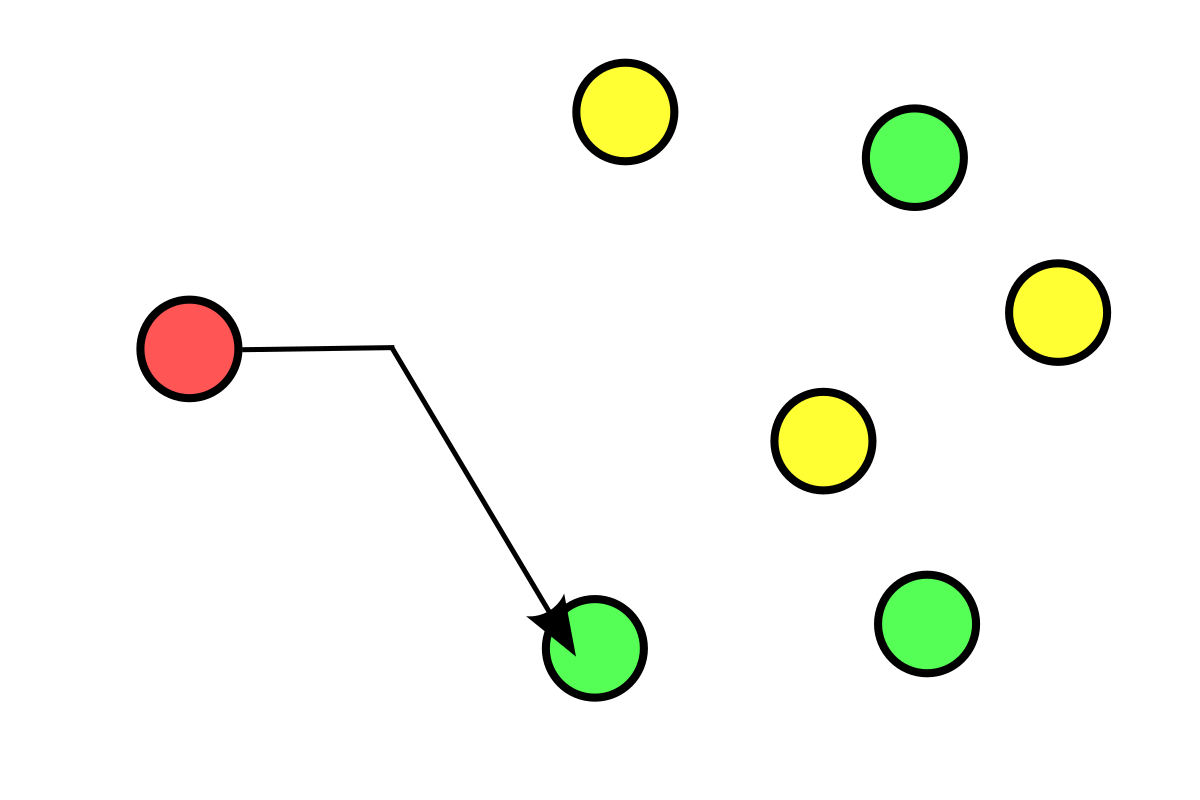
\includegraphics[width=0.5\textwidth]{images/ar.png}
    \caption{Anycast Routing}
\end{figure}
\newpage
% ========================== Routing for Mobile Hosts =============
\section*{Routing for Mobile Hosts}
Routing to Mobile Hosts (Mobile IP) Mobile IP is the primary mechanism in today's Internet architecture to tackle the problem of routing packets to mobile hosts. It introduces a few new capabilities but does not require any change from non-mobile hosts or most routers—thus making it incrementally deployable.

\newline The mobile host is assumed to have a permanent IP address, called its home address, which has a network prefix equal to that of its home network. This is the address that will be used by other hosts when they initially send packets to the mobile host; because it does not change, it can be used by long-lived applications as the host roams. We can think of this as the long-lived identifier of the host.

\newline When the host moves to a new foreign network away from its home network, it typically acquires a new address on that network using some means such as DHCP. This address is going to change every time the host roams to a new network, so we can think of this as being more like the locator for the host, but it is important to note that the host does not lose its permanent home address when it acquires a new address on the foreign network. This home address is critical to its ability to sustain communications as it moves, as we'll see below.
\begin{itemize}
    \item Mobile hosts introduce a new complication: to route a packet to a
mobile host, the network first has to find it.
    \item We will assume that all hosts are assumed to have a permanent
home location that never changes. Each hosts also has a permanent
home address that can be used to determine its home location.
    \item The routing goal is to make it possible to send packets to mobile
hosts using their fixed home addresses and have the packets efficiently
reach them wherever they may be.
    \item A different model would be to recompute routes as the mobile host
moves and the topology changes. We could then simply use the
routing schemes described earlier in this section. Any issues?
    \item Another alternative would be to provide mobility above the network
layer. When they are moved to new Internet locations, laptops
acquire new network addresses. In coming packets would need a
higher layer location service. Moreover, connections cannot be
maintained while the host is moving.
\end{itemize}

\newpage \begin{figure}
    \centering
    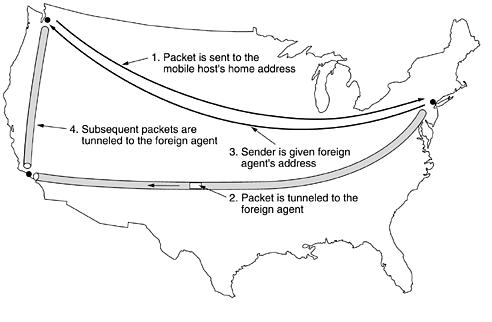
\includegraphics[width=\textwidth]{images/rfmh2.JPG}
    \caption{Routing for Mobile Hosts}
\end{figure}

% ========================== Routing for Adhoc Networks ============================
\section*{Routing for Adhoc Networks}
In adhoc networks, nodes are not familiar with the topology of their networks. Instead, they have to discover it: typically, a new node announces its presence and listens for announcements broadcast by its neighbors. Each node learns about others nearby and how to reach them, and may announce that it too can reach them. The difficulty of routing may be compounded by the fact that nodes may be mobile, which results in a changing topology.

\newline Adhoc routing protocols fall in two broad categories: proactive and reactive. Proactive or table-driven protocols maintain fresh lists of destinations and their routes by periodically distributing routing tables throughout the network. Reactive or on-demand protocols find a route on demand by flooding the network with Route Request packets.
\begin{itemize}
    \item We have now seen how to do routing when the hosts are mobile but the routers are fixed.
    \item Each node communicates wirelessly and acts as both a host and a router. Networks of nodes that just happen to be near each other are called ad hoc networks or MANETs (Mobile Ad hoc NETworks).
    \item Create multi-hop connectivity among set of
wireless, possibly moving, nodes.
    \item Mobile, wireless hosts act as forwarding nodes as
well as end systems
    \item Need routing protocol to find multi-hop paths
    \begin{itemize}
        \item Needs to be dynamic to adapt to new routes,
movement
        \item Interesting challenges related to interference and power limitations
        \item Low consumption of memory, bandwidth, power
        \item Scalable with numbers of nodes
        \item Localized effects of link failure
    \end{itemize}
    \item AODV(Ad hoc On-demand Distance Vector)
(Perkins and Royer, 1999)is a relative of the distance vector
algorithm that has been adapted to work in a mobile environment, in
which nodes often have limited bandwidth and battery lifetimes.
    \\
    Routes to a destination are discovered on demand, that is, only when a
somebody wants to send a packet to that destination.
\end{itemize}
\newline \begin{figure}
    \centering
    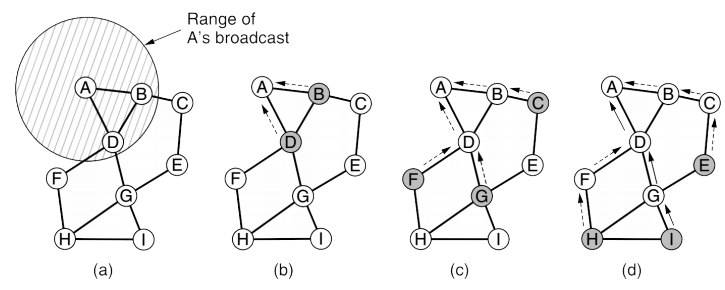
\includegraphics[width=\textwidth]{images/rfahn.png}
    \caption{Routing for Adhoc Networks}
\end{figure}
% \newpage
% ============================= Congestion Control =================================
\section*{Congestion Control}
Congestion is an important issue that can arise in packet switched network. Congestion is a situation in Communication Networks in which too many packets are present in a part of the subnet, performance degrades. Congestion in a network may occur when the load on the network (i.e. the number of packets sent to the network) is greater than the capacity of the network (i.e. the number of packets a network can handle.). Network congestion occurs in case of traffic overloading.
\begin{itemize}
    \item Too many packets present in (a part of) the network causes packet delay
and loss that degrades performance. This situation is called congestion.
The network and transport layers share the responsibility for handling
congestion.
\end{itemize}
\newpage  \begin{figure}
    \centering
    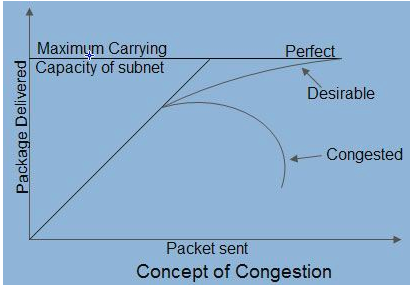
\includegraphics[width=\textwidth]{images/cc2.png}
    \caption{Congestion Control}
\end{figure}
\newpage
\newline The various causes of congestion in a subnet are:
\begin{itemize}
    \item The input traffic rate exceeds the capacity of the output lines. If suddenly, a stream of packet start arriving on three or four input lines and all need the same output line. In this case, a queue will be built up. If there is insufficient memory to hold all the packets, the packet will be lost. Increasing the memory to unlimited size does not solve the problem. This is because, by the time packets reach front of the queue, they have already timed out (as they waited the queue). When timer goes off source transmits duplicate packet that are also added to the queue. Thus same packets are added again and again, increasing the load all the way to the destination.
    \item The routers are too slow to perform bookkeeping tasks (queuing buffers, updating tables, etc.).
    \item The routers' buffer is too limited.
    \item Congestion in a subnet can occur if the processors are slow. Slow speed CPU at routers will perform the routine tasks such as queuing buffers, updating table etc slowly. As a result of this, queues are built up even though there is excess line capacity.
    
\end{itemize}
% \newpage
\\
\\
% ===================== Approaches to Congestion Control ===========================
\section*{Approaches to Congestion Control}
\begin{itemize}
    \item Congestion control has to do with making sure the network is able to
carry the offered traffic. It is a global issue, involving the behavior of all
the hosts and routers.
    \item Flow control, in contrast, relates to the traffic between a particular sender and a particular receiver. Its job is to make sure that a fast sender cannot continually transmit data faster than the receiver is able to absorb it.
    \item End-end congestion control
    \begin{itemize}
        \item no explicit feedback from network
        \item congestion inferred from end-system observed loss, delay
        \item approach taken by TCP
    \end{itemize}
    \item Network-assisted congestion control
    \begin{itemize}
        \item routers provide feedback to end systems
        \item single bit indicating congestion.
        \item explicit rate sender should send at
    \end{itemize}
\end{itemize}
\begin{figure}
    \centering
    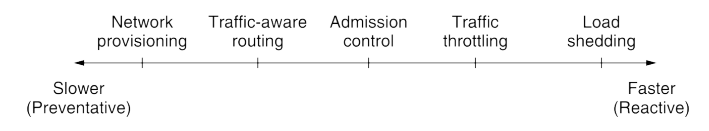
\includegraphics[width=\textwidth]{images/atcc.png}
    \caption{Approaches to Congestion Control}
\end{figure}
% \newpage
% ================Approaches to Congestion Control: Provisioning ===================
\newline \section*{Approaches to Congestion Control: Provisioning}
\begin{itemize}
    \item The most basic way to avoid congestion is to build a network that is
well matched to the traffic that it carries.
    \item If there is a low-bandwidth link on the path along which most traffic
is directed, congestion is likely. Sometimes resources can be added
dynamically when there is serious congestion, for example, turning on
spare routers or enabling lines that are normally used only as backups
(to make the system fault tolerant) or purchasing bandwidth on the
open market.
    \item More often, links and routers that are regularly heavily utilized are
upgraded at the earliest opportunity. This is called provisioning and
happens on a time scale of months, driven by long-term traffic trends.
    \item It is long term solution to congestion
    \item It involves :
    \begin{itemize}
        \item Spare routers
        \item Purchase extra bandwidth
        \item Allocate resources
    \end{itemize}
    \item Helps with temporary congestion conditions
\end{itemize}
% ========== Approaches to Congestion Control: Traffic-aware Routing ===============
\section*{Approaches to Congestion Control: Traffic-aware Routing}
Shifting traffic away from congested regions by setting the link weight to be a function of the link bandwidth and propagation delay plus the (variable) measured load or queuing delay.
\begin{itemize}
    \item To make the most of the existing network capacity, routes can be
tailored to traffic patterns that change during the day as network
users wake and sleep in different time zones.
    \item For example, routes may be changed to shift traffic away from heavily
used paths by changing the shortest path weights. This is called
traffic-aware routing.
    \item Splitting traffic across multiple paths is also helpful.
    \item The goal in taking load into-account when computing routes is to shift traffic away from hotspots.
    \item Least-weight paths will then favor paths.
\end{itemize}
\newline  \begin{figure}
    \centering
    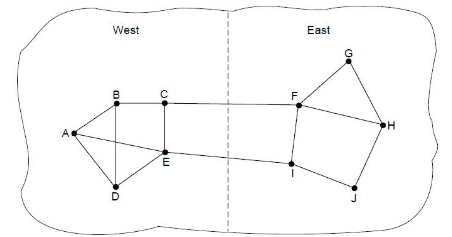
\includegraphics[width=\textwidth]{images/cct.png}
    \caption{Traffic-aware Routing : A Network in which the east and west parts are connected by two links}
\end{figure}
% =============================== References =====================================
\newpage \section*{References}
% \beginrefs
% \bibentry{AGM97}{\sc N.~Alon}, {\sc Z.~Galil} and {\sc O.~Margalit},
% On the Exponent of the All Pairs Shortest Path Problem,
% {\it Journal of Computer and System Sciences\/}~{\bf 54} (1997),
% pp.~255--262.

% \bibentry{F76}{\sc M. L. ~Fredman}, New Bounds on the Complexity of the 
% Shortest Path Problem, {\it SIAM Journal on Computing\/}~{\bf 5} (1976), 
% pp.~83-89.
% \endrefs
\begin{enumerate}
    \item \href{https://www.google.com/search?q=Routing+for+Mobile+Hosts&sxsrf=ACYBGNSF4TKefK2fJLrw0R5p1GUwwAmzJg:1569571775980&source=lnms&tbm=isch&sa=X&ved=0ahUKEwjwl6DBxvDkAhWOWX0KHWp0Ar4Q_AUIEigB&biw=1366&bih=586#imgrc=xAzmEaf0qCAsyM:}{Routing for Mobile Hosts}
    \item \href{https://www.google.com/search?q=Congestion+Control:+Traffic-aware+Routing&biw=1366&bih=637&sxsrf=ACYBGNQzEcKZZvweLk4Zfut06kaFYYka_w:1569569505171&source=lnms&tbm=isch&sa=X&ved=0ahUKEwjI8biGvvDkAhXNZSsKHVpPCCAQ_AUIEigB#imgrc=r5CN1cJ0IjvDCM:}{Traffic-aware Routing}
    \item \href{https://inet.omnetpp.org/docs/users-guide/ch-adhoc-routing.html}{Ad Hoc Routing}
    \item \href{http://ecomputernotes.com/computernetworkingnotes/communication-networks/what-is-congestion-control-describe-the-congestion-control-algorithm-commonly-used}{Congestion control}
    \item \href{https://www.google.com/search?biw=1366&bih=586&tbm=isch&sxsrf=ACYBGNQbbqG6czRopPGs9KzjIQ_sF0AmnQ%3A1569570980883&sa=1&ei=pMCNXca_NY3GvQSRtLjIAw&q=Approach+to+Congestion+Control&oq=Approach+to+Congestion+Control&gs_l=img.3..0i24.2660.2976..3272...0.0..0.102.291.1j2......0....1..gws-wiz-img.CZacXgpEAYQ&ved=0ahUKEwjGoY_Gw_DkAhUNY48KHREaDjkQ4dUDCAc&uact=5#imgrc=CoGZxgWLXWDKrM:}{Approach to Congestion Control}
    \item \href{http://bnrg.eecs.berkeley.edu/~randy/Courses/CS268.F09/lectures/12-adhocx2.pdf}{Ad Hoc Routing}
    \item \href{https://www.imperva.com/learn/performance/anycast/}{Anycast}
\end{enumerate}

\end{document}





